\documentclass{article}\usepackage[]{graphicx}\usepackage[]{color}
%% maxwidth is the original width if it is less than linewidth
%% otherwise use linewidth (to make sure the graphics do not exceed the margin)
\makeatletter
\def\maxwidth{ %
  \ifdim\Gin@nat@width>\linewidth
    \linewidth
  \else
    \Gin@nat@width
  \fi
}
\makeatother

\definecolor{fgcolor}{rgb}{0.345, 0.345, 0.345}
\newcommand{\hlnum}[1]{\textcolor[rgb]{0.686,0.059,0.569}{#1}}%
\newcommand{\hlstr}[1]{\textcolor[rgb]{0.192,0.494,0.8}{#1}}%
\newcommand{\hlcom}[1]{\textcolor[rgb]{0.678,0.584,0.686}{\textit{#1}}}%
\newcommand{\hlopt}[1]{\textcolor[rgb]{0,0,0}{#1}}%
\newcommand{\hlstd}[1]{\textcolor[rgb]{0.345,0.345,0.345}{#1}}%
\newcommand{\hlkwa}[1]{\textcolor[rgb]{0.161,0.373,0.58}{\textbf{#1}}}%
\newcommand{\hlkwb}[1]{\textcolor[rgb]{0.69,0.353,0.396}{#1}}%
\newcommand{\hlkwc}[1]{\textcolor[rgb]{0.333,0.667,0.333}{#1}}%
\newcommand{\hlkwd}[1]{\textcolor[rgb]{0.737,0.353,0.396}{\textbf{#1}}}%
\let\hlipl\hlkwb

\usepackage{framed}
\makeatletter
\newenvironment{kframe}{%
 \def\at@end@of@kframe{}%
 \ifinner\ifhmode%
  \def\at@end@of@kframe{\end{minipage}}%
  \begin{minipage}{\columnwidth}%
 \fi\fi%
 \def\FrameCommand##1{\hskip\@totalleftmargin \hskip-\fboxsep
 \colorbox{shadecolor}{##1}\hskip-\fboxsep
     % There is no \\@totalrightmargin, so:
     \hskip-\linewidth \hskip-\@totalleftmargin \hskip\columnwidth}%
 \MakeFramed {\advance\hsize-\width
   \@totalleftmargin\z@ \linewidth\hsize
   \@setminipage}}%
 {\par\unskip\endMakeFramed%
 \at@end@of@kframe}
\makeatother

\definecolor{shadecolor}{rgb}{.97, .97, .97}
\definecolor{messagecolor}{rgb}{0, 0, 0}
\definecolor{warningcolor}{rgb}{1, 0, 1}
\definecolor{errorcolor}{rgb}{1, 0, 0}
\newenvironment{knitrout}{}{} % an empty environment to be redefined in TeX

\usepackage{alltt}
\usepackage{amsmath}
\usepackage{makecell}
\setcellgapes{5pt}
\usepackage{graphics}
\usepackage{multicol}
\usepackage[cm]{fullpage}
\graphicspath{ {./images/} }
\usepackage{titling}

\title{COSC 6323 - Statistical Methods in Research\\Project Phase - 1\\}

\author{%
    Members: Team-8 \\\\
    1. Md Rafiqul Islam Rabin, \texttt{ID:1797648}, \texttt{mrabin@central.uh.edu}\vspace{2pt} \\
    2. Salah, \texttt{ID:}, \texttt{@}\vspace{2pt} \\
    3. Farah, \texttt{ID:}, \texttt{@}\vspace{2pt} \\
}

\date{March 08, 2019.}
\IfFileExists{upquote.sty}{\usepackage{upquote}}{}
\begin{document}

\maketitle
\par{\textbf{Contributions}: In the first week of the project, we worked on Fig 3. At first, we drew Fig 3 with ggplot, but as we faced a problem with y-log transformation, we moved to plot\_ly. We all equally contributed to Fig 3. After that, we sit together several times to discuss the required data for Gephi and Supplementary plot. Then we individually collect data (i.e. XDIndicator, Node, Edge, Etc.) from given CSV files. We cross-checked our data for confirmation. So, we all also equally contributed to the data processing. Now, at that moment, we divided our remaining tasks among us: 2B and S2 for Rabin, 2A and S4 for Farah, S1 and S3 for Salah. Although we divided our tasks at that stage, we always shared our progress/problem and helped each other during implementation. We created a git repository and distributively contributed for the project. As we all completed our tasks and actively involved with each other all the times, we almost equally contributed to this phase of project. Here is the overall contribution percentage: Rabin(35\%), Farah(33\%) and Salah(32\%).}

%Fig. 2A
\newpage
\section*{\underline{Fig. 2(A) :}}
\begin{center}
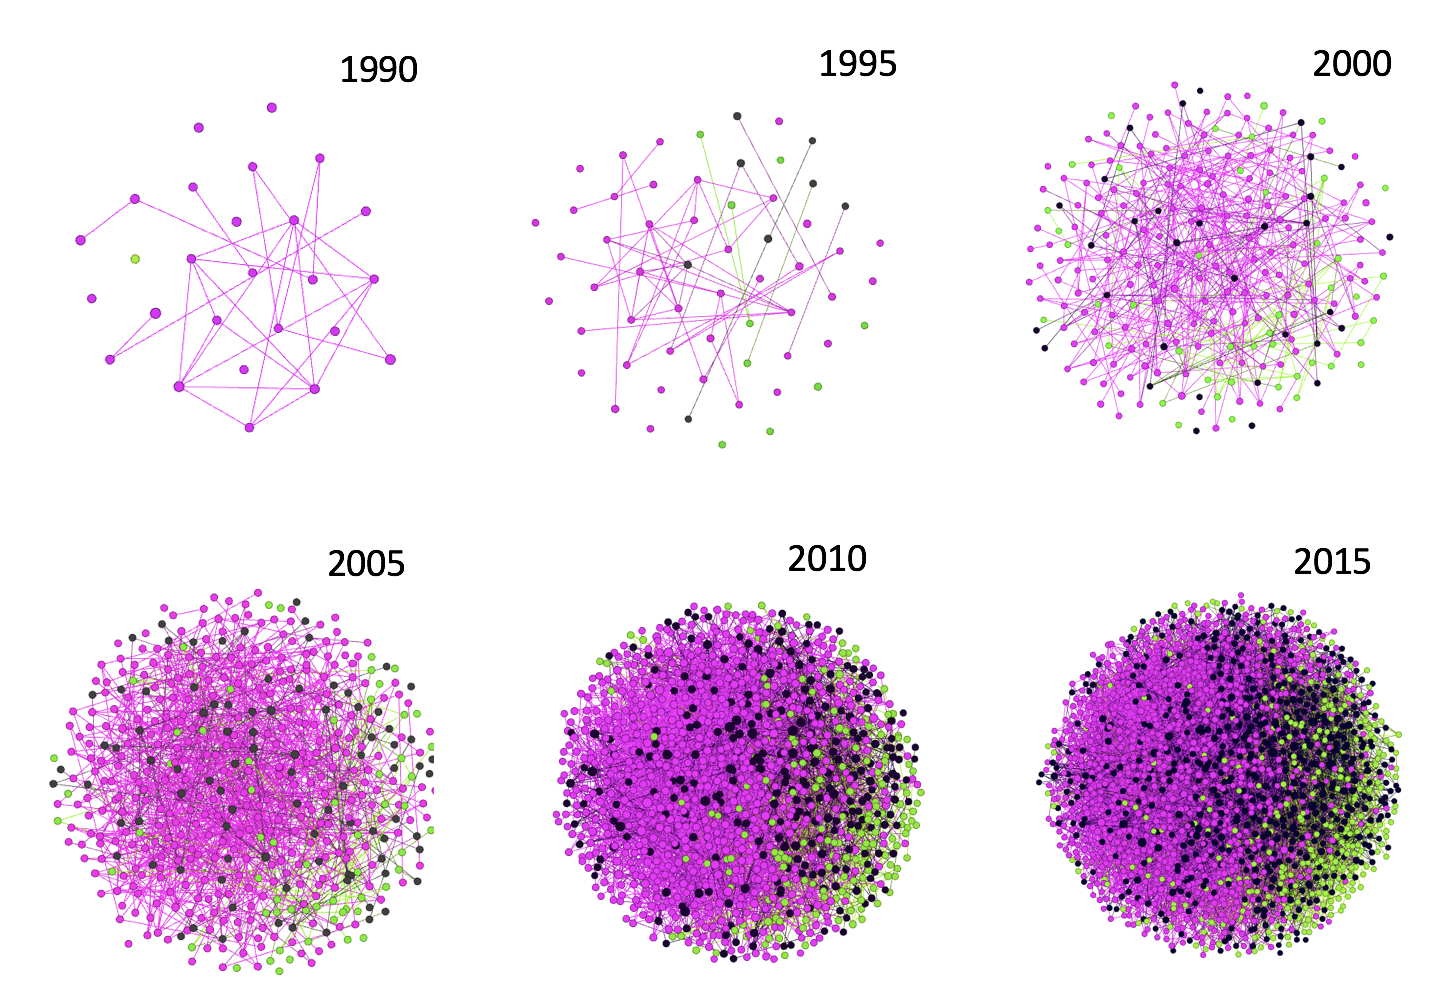
\includegraphics[scale=0.6]{2A.png}
\newline
\par{\textbf{Fig. 2. Growth of cross-disciplinary social capital.} 
\textbf{(A)} Evolution of the giant component in the U.S. biology-computing network.}
\end{center}
\subsection*{\underline{Description of figure content:}}
\par{Here, ...}
\subsection*{\underline{Observations, conclusions, and hypotheses:}}
\par{Here, ...}

%Fig. 2B
\newpage
\section*{\underline{Fig. 2(B) :}}
\begin{center}
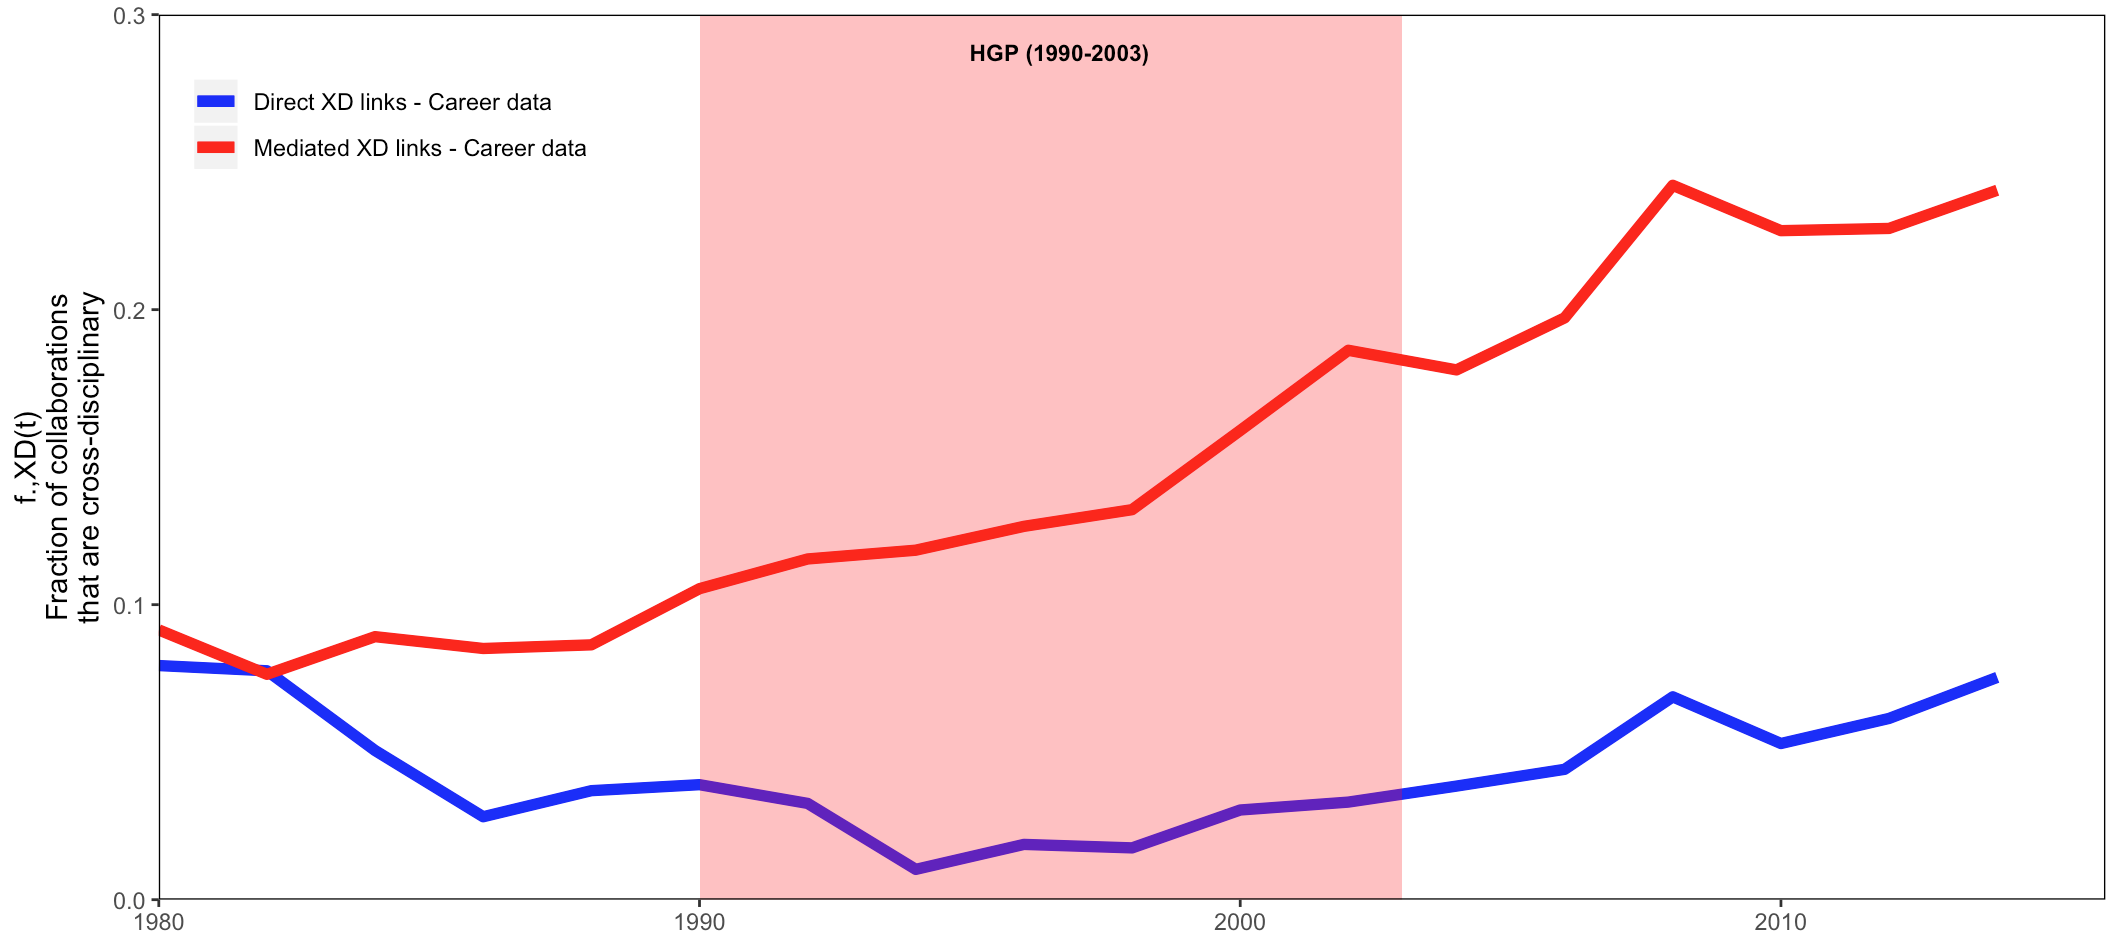
\includegraphics[scale=0.4]{2B.png}
\newline
\par{\textbf{Fig. 2. Growth of cross-disciplinary social capital.} \textbf{(B)} Evolution of the fraction of collaboration links in the \textit{F} network that are cross-disciplinary.}
\end{center}
\subsection*{\underline{Description of figure content:}}
\par{Here, in Fig 2B, we plotted the fraction of cross-disciplinary collaboration for each nonoverlapping 2-years period through (1979-1980) to (2013-2014). The blue and red line represents the trend of Direct-XD links and Mediated-XD links, respectively. For each nonoverlapping 2-years period, we collected all the publication data from \textbf{GoogleScholar\_paper\_stats.csv} file. Then, for the Direct-XD links, we count total direct (F-F) links and total cross-discipline direct links for each period. Finally, we calculated the fraction of direct cross-disciplinary collaboration by \textbf{total F-F direct links / total cross-discipline direct links}. Similarly, for the Mediated-XD links, we count total mediated (F-P-F) links and cross-discipline mediated links for each period. Finally, we calculated the fraction of mediated cross-disciplinary collaboration by \textbf{total F-P-F mediated links / total cross-discipline mediated links.}}
\subsection*{\underline{Observations, conclusions, and hypotheses:}}
\begin{description}
  \item[$\bullet$] The first thing we can see that, the growth is comparatively higher for mediated cross-disciplinary collaboration but slower for direct cross-disciplinary collaboration. This highlights that pollinators are more likely to be cross link than direct faculty persons.
  \item[$\bullet$] Both the direct and mediated cross-disciplinary collaboration has increased during HGP(1990-2003) period and the increasing rate also continues upward after the HGP as well. So, the impact of HGP on cross-disciplinary collaboration is clearly visible.
  \item[$\bullet$] The increasing rate of cross-disciplinary collaboration continues. In recent years (i.e. by 2015) the direct cross-disciplinary collaboration becomes almost 10\% of total direct collaboration, and the mediated cross-disciplinary collaboration becomes almost 30\% of total mediated collaboration (whether within-discipline or cross-discipline).
\end{description}

%Fig. 3
\newpage
\section*{\underline{Fig. 3 :}}
\begin{center}
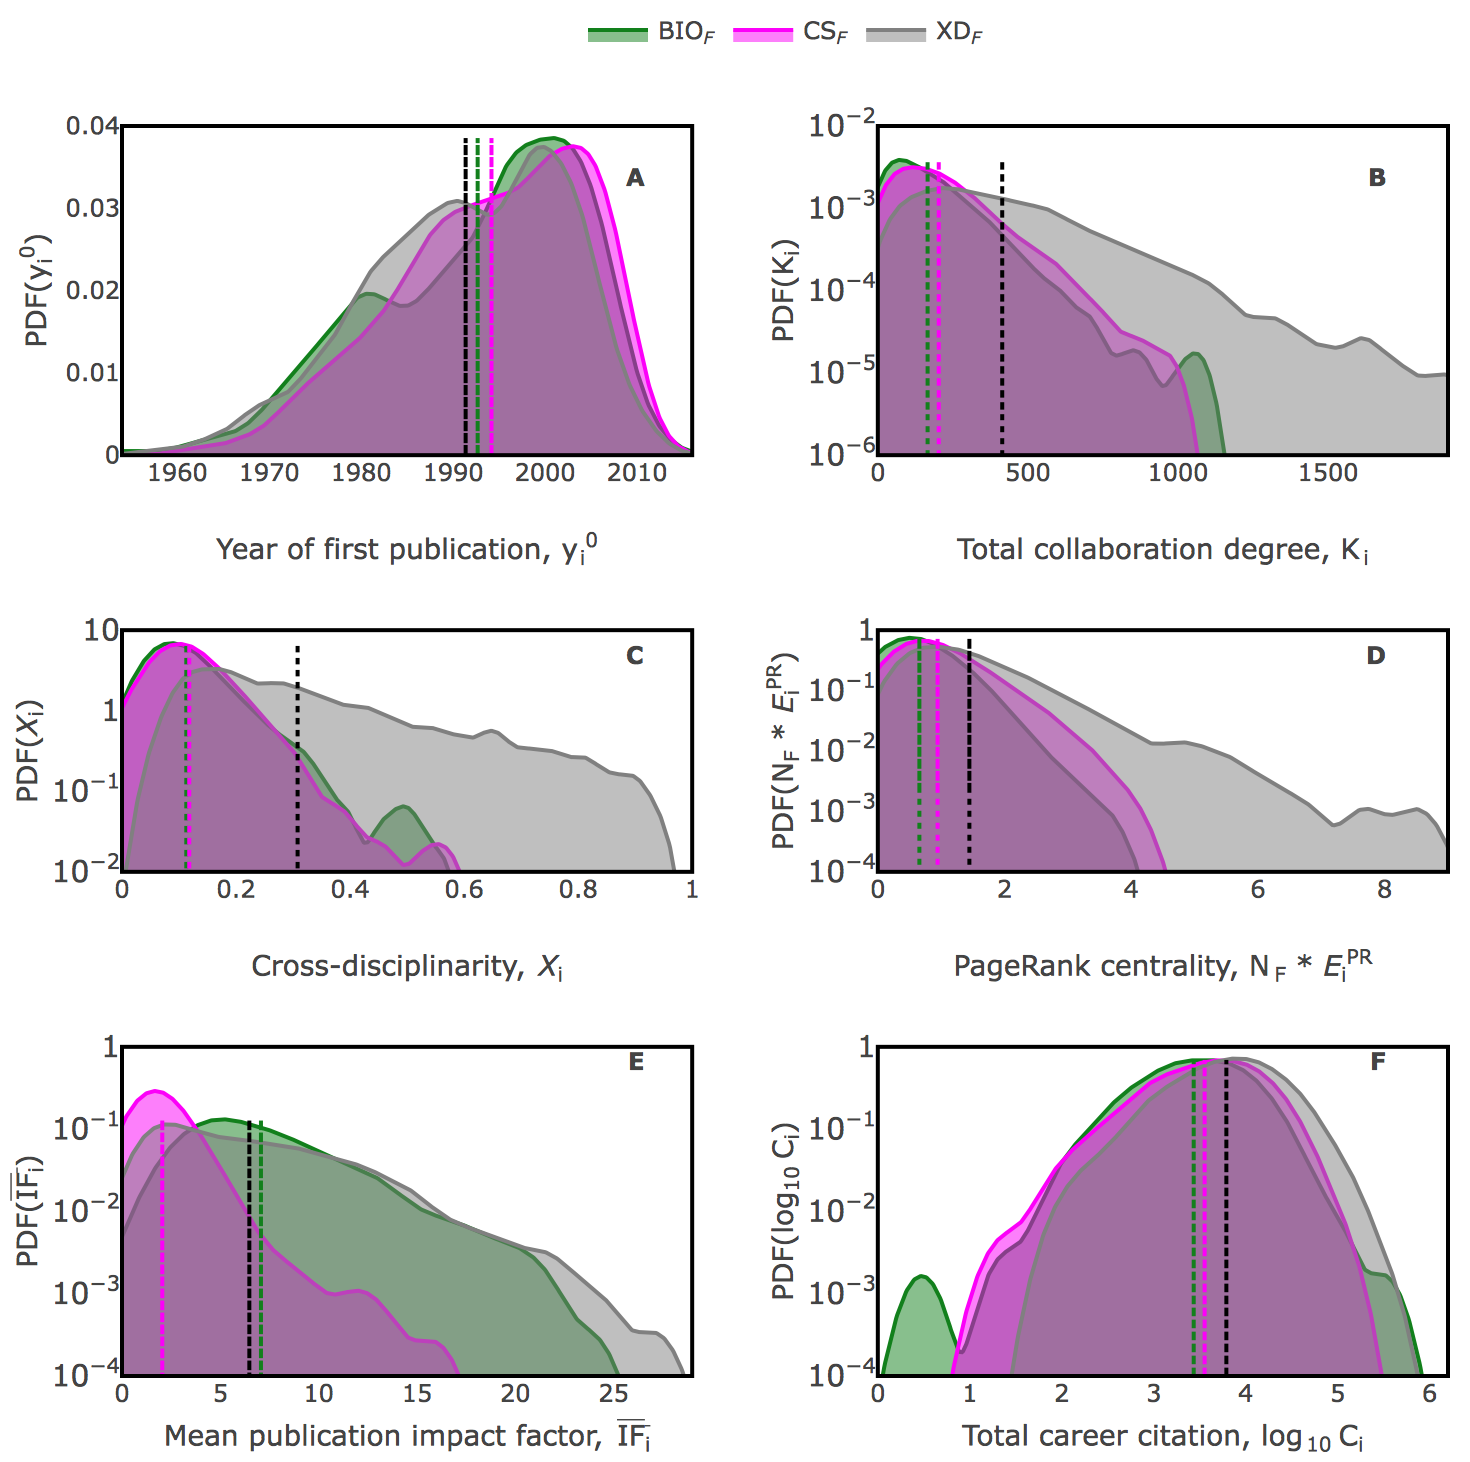
\includegraphics[scale=0.6]{3.png}
\newline
\par{\textbf{Fig. 3. Descriptive statistics for the career data set.}}
\end{center}
\subsection*{\underline{Description of figure content:}}
\par{In Fig-3, Green color represents the Biology, Majenta color represents Computer Science, and Gray color represents the Cross-platform distributions. The vertical lines denote the mean values of the corresponding distribution. The Fig-A describes the probability distribution of the year of first publication, yi0, by faculty members. Fig-B, the probability distribution of a total number of collaborators for each faculty member. Fig-C describes the ratio of cross-disciplinary collaborator faculties. Fig-D, the probability distribution for page rank centrality, where NF describes the number of faculty members in the corresponding department. Fig-E, the probability distribution of mean impact factor, IFi, of publications of faculty members. Fig-F describes the probability distribution of total citations of each faculty member in log10 scale.}
\subsection*{\underline{Observations, conclusions, and hypotheses:}}
\begin{description}
  \item In Fig-3, we have several statistical comparisons on research activities among Biology (BIO), Computer Science (CS), and Cross-Platform (XD) faculty members. 
  \item[$\bullet$] In Fig-A, we can see that the average starting publication time in the early 1990s. The rate of adding new professors in research in all platforms are similar. 
  \item[$\bullet$]Fig-B shows that Cross-platform (XD) faculty members have a significantly higher number of collaborations than Computer Science (CS) or Biology (BIO) groups. 
  \item[$\bullet$]Fig-C indicates that the Cross-platform (XD) group has a significantly higher degree of cross-disciplinarity (Xi) than the other two groups.
  \item[$\bullet$]Fig-D shows that the mean centrality value for google page rank is significantly higher in cross-disciplinary faculty members than other groups. 
  \item[$\bullet$]Fig-E shows the mean publication impact factor. The figure shows that the Biology and Cross-disciplinary groups have similar publishing pattern.
  \item[$\bullet$]In Fig-F, we can see that the mean value of total career citations is similar in all disciplinary faculty members.
\end{description}


%Fig. S1
\newpage
\section*{\underline{Fig. S1 :}}
\begin{center}
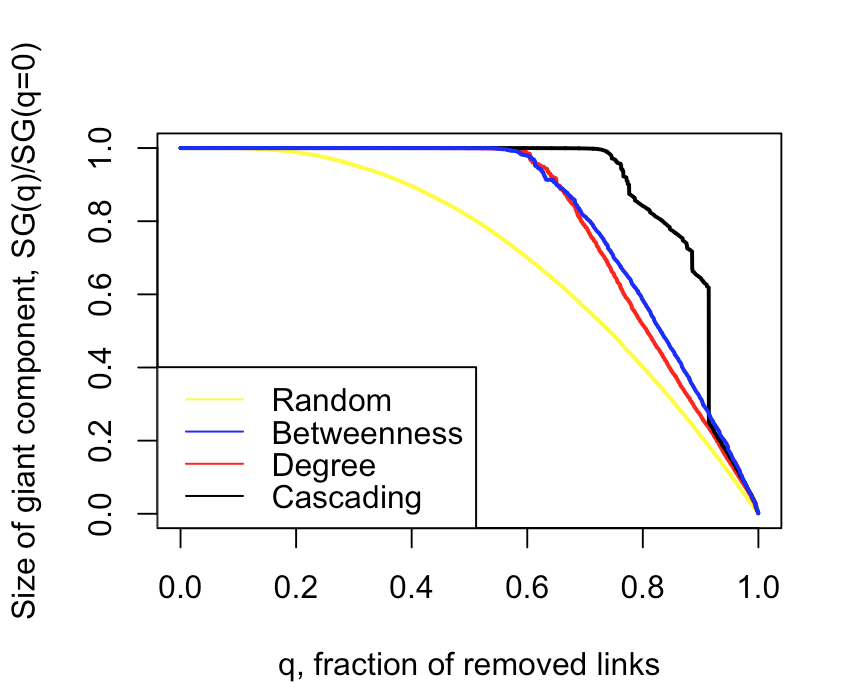
\includegraphics[scale=0.4]{S1.png}
\newline
\par{\textbf{Fig. S1. Robustness of the F network with respect to link removal.}}
\end{center}
\subsection*{\underline{Description of figure content:}}
\par{Here, ...}
\subsection*{\underline{Observations, conclusions, and hypotheses:}}
\par{Here, ...}

%Fig. S2
\newpage
\section*{\underline{Fig. S2 :}}
\begin{center}
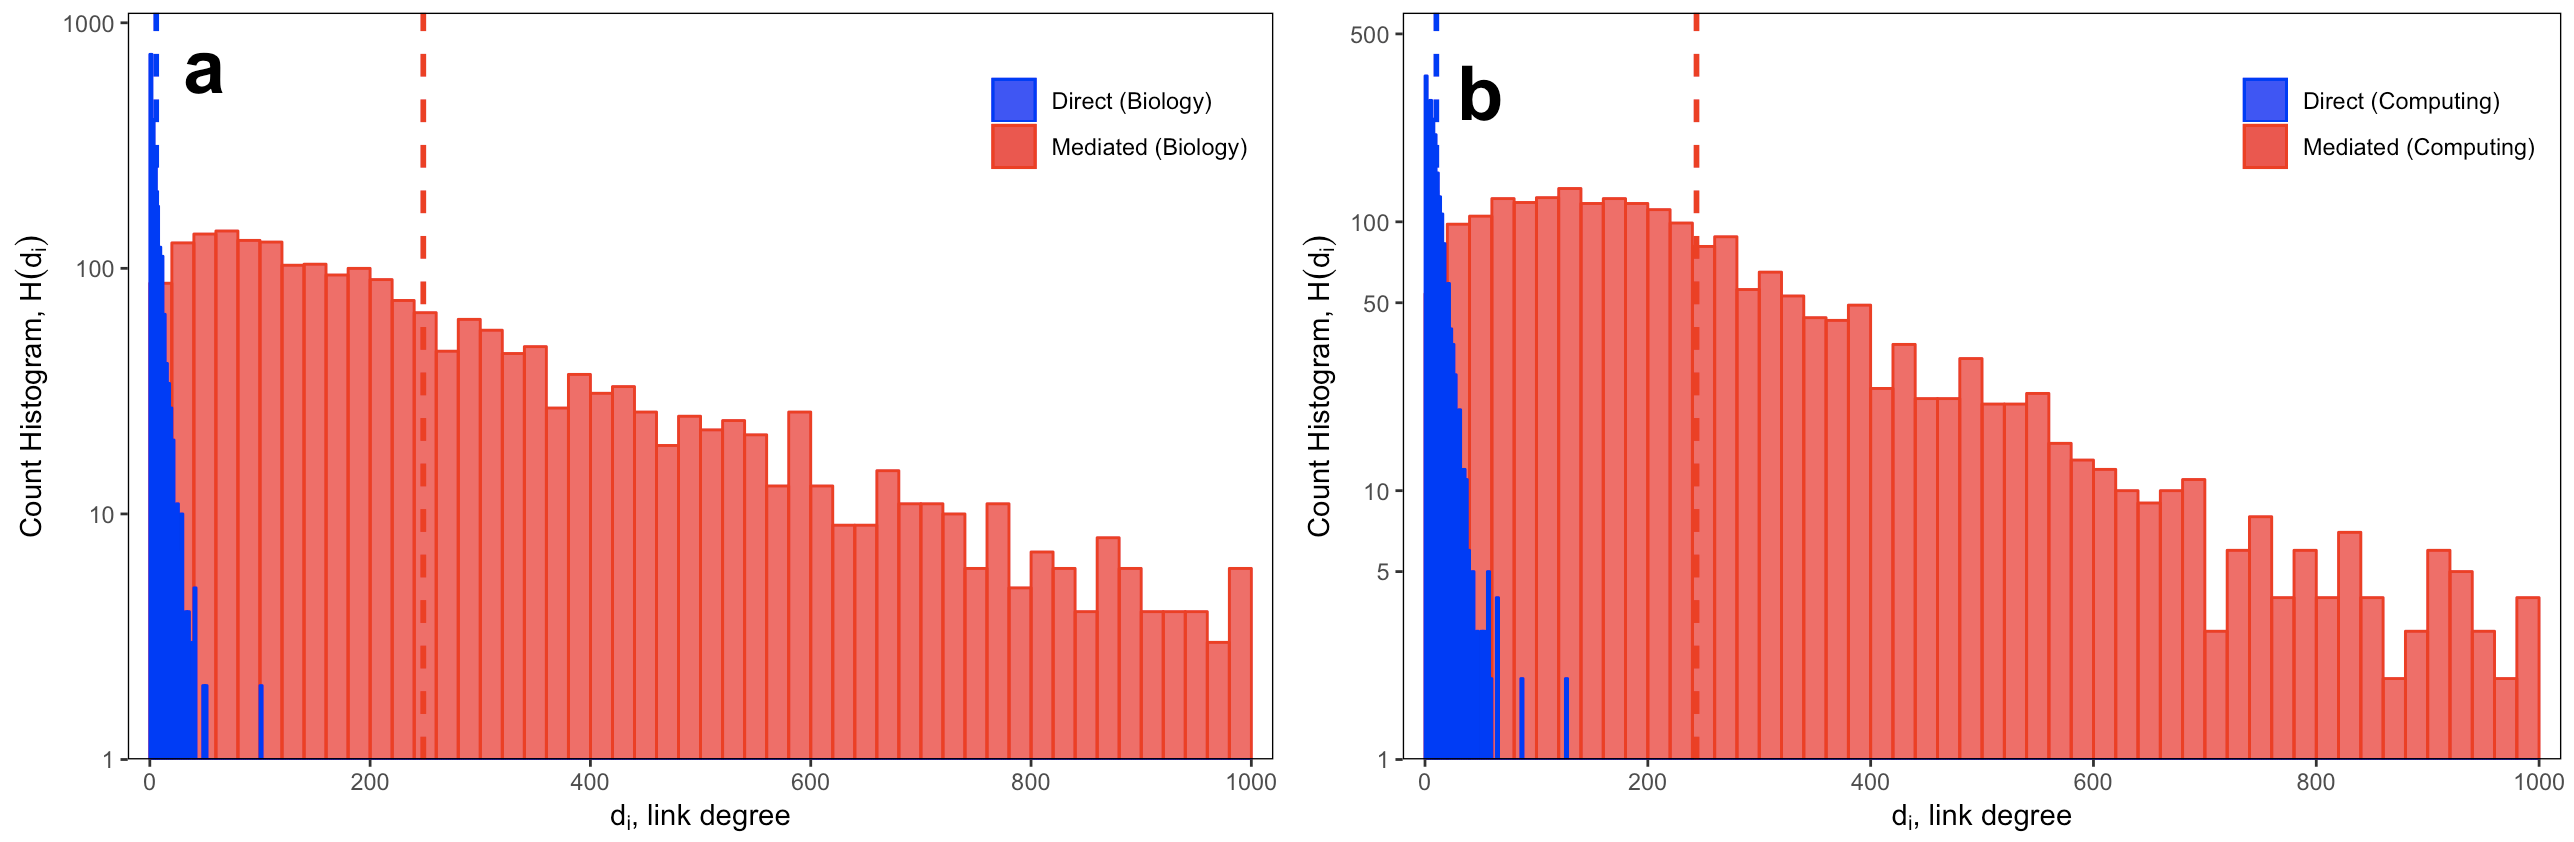
\includegraphics[scale=0.45]{S2.png}
\newline
\par{\textbf{Fig. S2. \textit{F} network distributions for direct and mediated associations.}}
\end{center}
\subsection*{\underline{Description of figure content:}}
\par{Here, in Fig S2, we showed the frequency distribution (counts) of faculty within a given link degree. Histogram \textbf{(a)} for biology department and \textbf{(b)} for computing department. At first, we read the \textbf{KDirect} and \textbf{KMediated} data from \textbf{Faculty\_GoogleScholar\_Funding\_Data\_N4190.csv} file for \textbf{BIO} and \textbf{CS} department, separately. Then we used binwidth=20 for mediated counts and binwidth=2 for direct counts, for both biology and computing department. The blue and red bar represent the counts for direct and mediated links, respectively. The blue and red vertical lines indicate the distribution means for direct and mediated links, respectively.}
\subsection*{\underline{Observations, conclusions, and hypotheses:}}
\begin{description}
  \item[$\bullet$] In higher link degree (i.e after 200 link degree), the mediated link counts are still significant but there is almost no direct link counts, for both biology and computing department. 
  \item[$\bullet$] More than 90\% co-authors are pollinators, for both biology and computing department. 
  \item[$\bullet$] The mean line, for both biology and computing department, clearly shows that the mediated link degree are higher than the direct link degree. 
  \item[$\bullet$] Finally, the significant impact of pollinators in network distributions is clearly visible.
\end{description}

%Fig. S3
\newpage
\section*{\underline{Fig. S3 :}}
\begin{center}
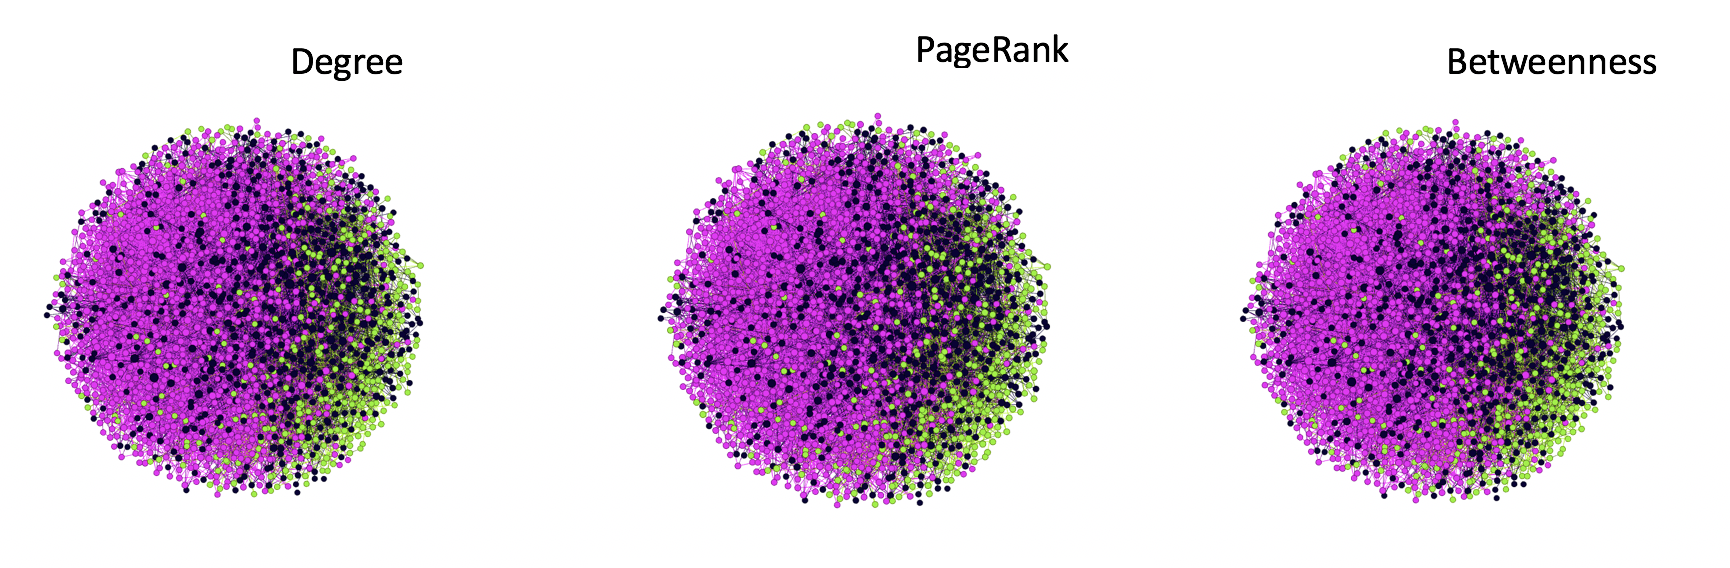
\includegraphics[scale=0.5]{S3.png}
\newline
\par{\textbf{Fig. S3. Three perspectives on the centrality of F\textsubscript{i} in the direct collaboration network.}}
\end{center}
\subsection*{\underline{Description of figure content:}}
\par{Here, ...}
\subsection*{\underline{Observations, conclusions, and hypotheses:}}
\par{Here, ...}

%Fig. S4
\newpage
\section*{\underline{Fig. S4 :}}
\begin{center}
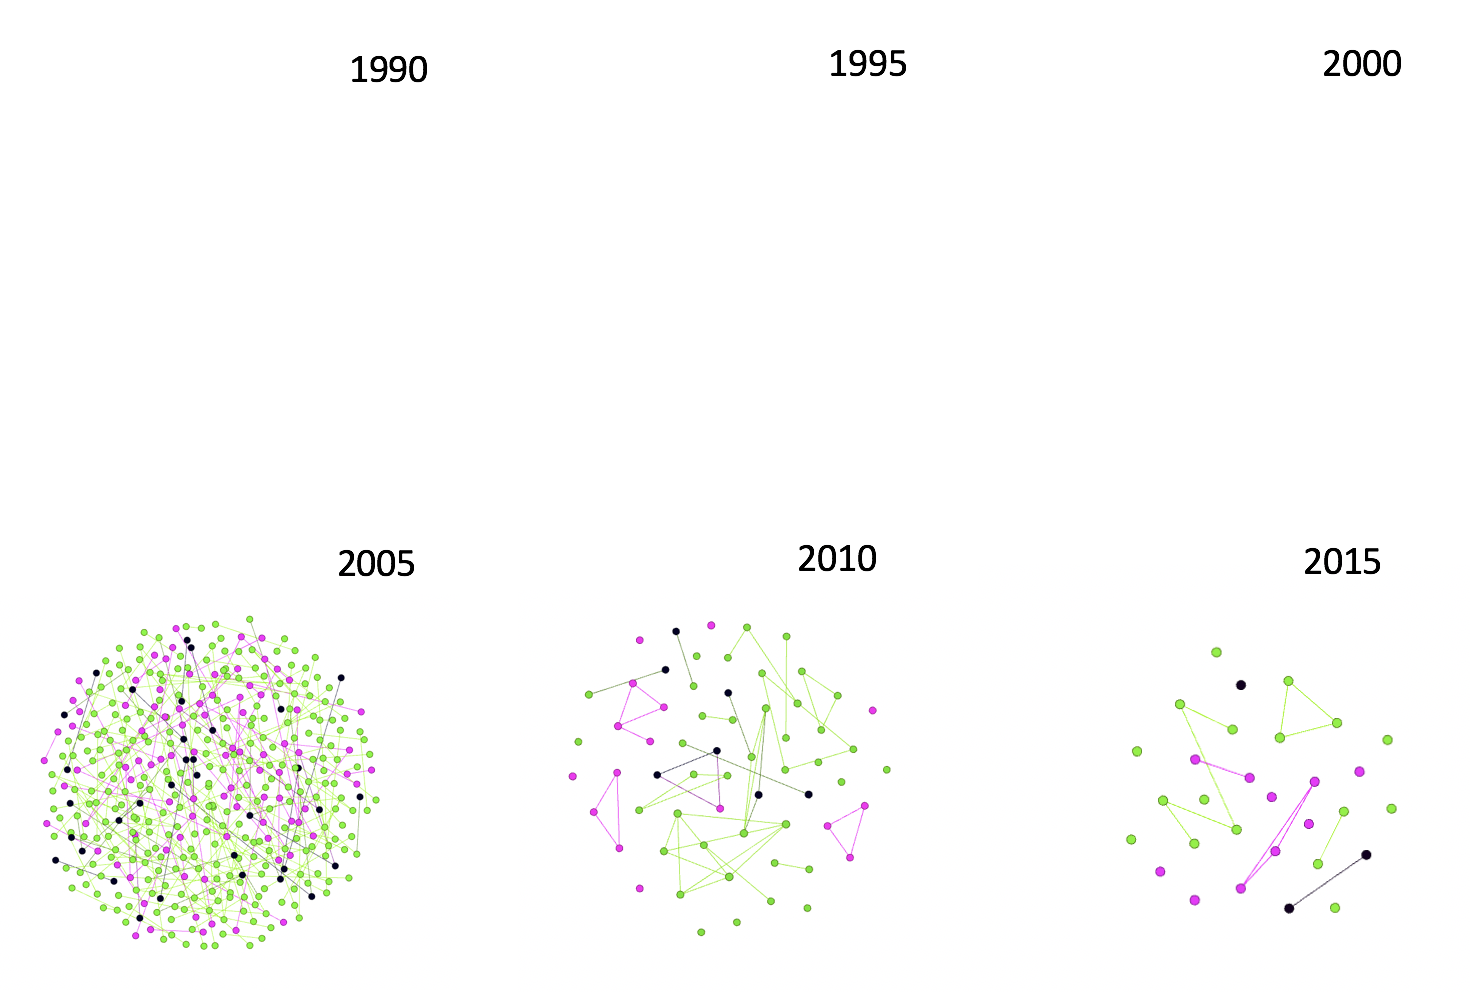
\includegraphics[scale=0.6]{S4.png}
\newline
\par{\textbf{Fig. S4. Evolution of the nongiant components in the F network.}}
\end{center}
\subsection*{\underline{Description of figure content:}}
\par{Here, ...}
\subsection*{\underline{Observations, conclusions, and hypotheses:}}
\par{Here, ...}

\end{document}
